\documentclass[tikz,border=4pt]{standalone}
\usepackage{tikz}
\usetikzlibrary{arrows.meta,patterns}
\begin{document}
\begin{tikzpicture}[>=Stealth]
    \node[font=\bfseries] at (3,3.5) {Conditional Probability};

    % Sample space rectangle
    \draw[thick,rounded corners=3pt] (0,0) rectangle (6,3);

    % Event B ellipse
    \draw[blue!60,fill=blue!15,thick] (3.5,1.5) ellipse (2.2 and 1.2);
    \node[blue!70,font=\bfseries] at (4.8,2.5) {$B$};

    % Event A ellipse
    \draw[red!60,fill=red!15,thick] (2.5,1.5) ellipse (1.8 and 1.1);
    \node[red!70,font=\bfseries] at (1.2,2.4) {$A$};

    % Intersection label
    \node[font=\small,purple!70] at (3,1.5) {$A \cap B$};

    % Sample space label
    \node[gray,font=\small] at (5.5,0.3) {$\Omega$};

    % Formula
    \node[font=\small,anchor=north] at (3,-0.4)
        {$P(A \mid B) = \dfrac{P(A \cap B)}{P(B)}$};
\end{tikzpicture}
\end{document}
